\begin{center}
    \chapter{Literature Review}
\end{center}
\label{chap:litreview}

\noindent
Electricity demand forecasting is a core requirement for modern power systems because operators must continuously balance generation and consumption, schedule reserves, and manage market commitments under uncertainty~\cite{hong2016probabilistic}. The transition to renewable-heavy grids increases this difficulty: variable generation, weather-sensitive demand, and market volatility make deterministic planning less reliable. For this reason, this project focuses on \emph{probabilistic short-term demand forecasting}, where forecasts are not only accurate on average but also informative about uncertainty.

\noindent
This chapter first presents the general methodological background of electricity demand forecasting, then focuses on the target paper by Smyl et al.~\cite{smyl2025anyquantile}, \emph{Any-quantile probabilistic forecasting of short-term electricity demand: Fusing uncertainties from diverse sources}. In line with the project scope, metric discussion and mathematical formalism are intentionally minimized.

\section{Technical Background}
\label{sec:techbg}

\subsection{Methodologies for Electricity Demand Forecasting}
\label{subsec:method_overview}

The literature usually organizes short-term demand forecasting methods into four families:
\begin{itemize}
    \item \textbf{Classical statistical models} (e.g., ARIMA, exponential smoothing): strong baselines for stable seasonal patterns, but less effective when demand dynamics become highly nonlinear.
    \item \textbf{Machine-learning models} (e.g., quantile regression, boosting): more flexible with nonlinear effects and interactions, but often sensitive to feature engineering and data shifts.
    \item \textbf{Deep learning models} (e.g., DeepAR, WaveNet, TFT, N-BEATS): strong representation capacity for multi-scale temporal structure and exogenous drivers.
    \item \textbf{Post-hoc uncertainty calibration methods} (e.g., conformal prediction/CQR): used to improve interval reliability without retraining the full forecaster~\cite{vovk2005,romano2019cqr}.
\end{itemize}

Across these families, exogenous information (especially weather and calendar variables) is a major performance driver in load forecasting~\cite{hong2016probabilistic}. Recent work therefore focuses not only on architecture design, but also on how to \emph{fuse} multiple uncertainty sources: historical demand variability, weather uncertainty, and model uncertainty.

\subsection{Minimal Evaluation Perspective}
\label{subsec:min_metrics}

For probabilistic forecasting, most studies report distribution-quality metrics such as CRPS and interval coverage; point metrics (e.g., MAE/MAPE) are usually evaluated on a central estimate such as the median forecast~\cite{gneiting2007strictly}. In this chapter, metrics are used only as contextual indicators of comparative performance, not as a theoretical focus.

\subsection{Architectural Basis: N-BEATS and Any-Quantile Extension}
\label{subsec:arch_basis}

N-BEATS is a deep residual architecture designed for time-series forecasting with strong empirical performance and a simple fully connected design~\cite{oreshkin2020nbeats}. Smyl et al.~\cite{smyl2025anyquantile} build on this foundation and introduce an \emph{any-quantile} mechanism: one model can produce forecasts for arbitrary quantile levels at inference time.

Conceptually, this extension conditions the network on the requested quantile level and learns a unified mapping from input history (plus exogenous context) to quantile outputs. This is operationally attractive because it avoids training separate models for each quantile.

In the main paper, three AQ-NBEATS variants are presented~\cite{smyl2025anyquantile}:
\begin{itemize}
    \item \textbf{AQ-CAT}: the target quantile level is concatenated with the input representation. This is the simplest conditioning strategy and has low implementation complexity.
    \item \textbf{AQ-FiLM}: the quantile level modulates intermediate hidden representations through feature-wise affine transformations (FiLM-style conditioning). This is more expressive, because conditioning acts inside the network, not only at the input.
    \item \textbf{AQ-OUT}: the quantile level is injected at the output stage. This keeps the shared backbone largely unchanged while allowing quantile-specific output behavior.
\end{itemize}

The three designs trade off simplicity, expressiveness, and computational efficiency. AQ-CAT is usually the lightest to implement, AQ-FiLM offers richer internal conditioning, and AQ-OUT provides a compromise by concentrating quantile adaptation near the final prediction layer. Their architectural differences are illustrated in Figures~\ref{fig:aq_cat_arch}, \ref{fig:aq_film_arch}, and~\ref{fig:aq_out_arch}.

\begin{figure}[H]
    \centering
    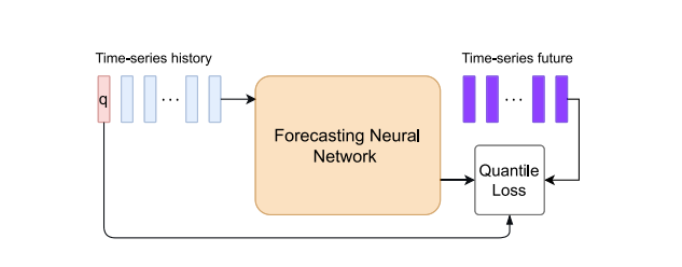
\includegraphics[width=0.85\textwidth]{images/aq-cat.png}
    \caption{AQ-CAT architecture (adapted from Smyl et al.~\cite{smyl2025anyquantile}).}
    \label{fig:aq_cat_arch}
\end{figure}

\begin{figure}[H]
    \centering
    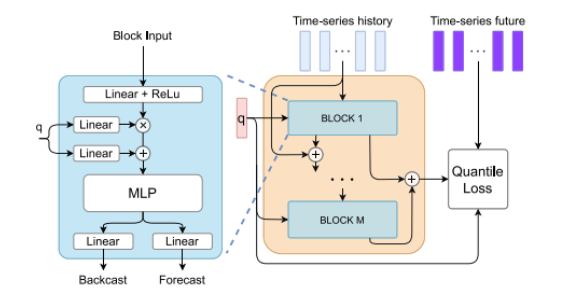
\includegraphics[width=0.85\textwidth]{images/aq_film.png}
    \caption{AQ-FiLM architecture (adapted from Smyl et al.~\cite{smyl2025anyquantile}).}
    \label{fig:aq_film_arch}
\end{figure}

\begin{figure}[H]
    \centering
    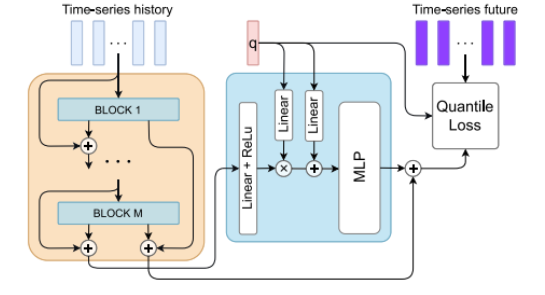
\includegraphics[width=0.85\textwidth]{images/aq-out.png}
    \caption{AQ-OUT architecture (adapted from Smyl et al.~\cite{smyl2025anyquantile}).}
    \label{fig:aq_out_arch}
\end{figure}

\section{Focused Study: Smyl et al. (2026)}
\label{sec:smyl_focus}

\subsection{Problem Framing and Methodological Contribution}
\label{subsec:smyl_contribution}

Smyl et al.~\cite{smyl2025anyquantile} address short-term electricity demand forecasting as a probabilistic task where different uncertainty sources must be represented coherently. Their key contribution is a practical any-quantile framework based on AQ-NBEATS and related variants, enabling dense quantile generation from a single trained model.

\subsection{Models Used in the Study}
\label{subsec:smyl_models}

The paper compares classical, machine-learning, and deep-learning baselines with any-quantile models. The reported benchmark set includes Naive, ARIMA, ES, Theta, quantile regression (QR), NGBoost, MLP, DeepAR, WaveNet, Transformer, TFT, AQ-ESRNN, and AQ-NBEATS~\cite{smyl2025anyquantile}. For this project, the most important models are AQ-ESRNN and AQ-NBEATS:

\begin{itemize}
    \item \textbf{AQ-ESRNN}: extends the ES-RNN family by combining exponential-smoothing style level/seasonality handling with a neural component, then producing quantiles through the any-quantile conditioning mechanism. Its main strength is robust handling of strong seasonality with probabilistic outputs from a single model.
    \item \textbf{AQ-NBEATS}: adapts the N-BEATS residual block architecture to quantile conditioning, so the model can generate arbitrary quantile forecasts at inference time. Its main strength is high flexibility for complex nonlinear demand patterns while avoiding one-model-per-quantile training.
\end{itemize}

In the benchmark reported by Smyl et al.~\cite{smyl2025anyquantile}, AQ-NBEATS is central for capturing multi-scale demand dynamics, while AQ-ESRNN provides a strong seasonal probabilistic baseline. This complementarity is important for the design of our staged combined solution in later chapters.

\subsection{Dataset Used}
\label{subsec:smyl_data}

The core benchmark dataset is \textbf{EMHIRES} (short-term electricity demand across 35 European countries, hourly resolution), with associated time/context information used for forecasting experiments in the paper~\cite{smyl2025anyquantile}. This dataset choice is important because it reflects heterogeneous national demand scales and seasonality patterns, making uncertainty-aware evaluation meaningful.

\subsection{Main Limitation and Suggested Direction}
\label{subsec:smyl_limits}

From the reviewed studies, and especially from the deployment perspective of any-quantile deep models, the main limitations are:
\begin{itemize}
    \item \textbf{Dependence on exogenous quality}: weather and calendar inputs are often decisive for short-term load forecasting quality; missing values, noisy weather estimates, or weak feature alignment can degrade both point accuracy and quantile reliability~\cite{hong2016probabilistic}.
    \item \textbf{Calibration fragility under regime shifts}: sudden demand-pattern changes (policy changes, extreme weather, behavioral shifts) can reduce probabilistic calibration even when average error remains acceptable.
    \item \textbf{Model transferability limits}: models trained on heterogeneous countries may not transfer equally across all local demand structures; robustness can vary across regions and seasons.
    \item \textbf{Operational interpretability constraints}: deep probabilistic outputs are useful for decision support, but explaining why specific quantile bands widen or narrow is still less transparent than with simpler statistical baselines.
\end{itemize}

A direct methodological direction is to combine strong any-quantile backbones (especially AQ-NBEATS and AQ-ESRNN) with adaptive post-hoc recalibration, such as conformalized quantile regression (CQR), and with shift-aware updating policies to preserve reliability over time~\cite{romano2019cqr}.
\section{Related Studies: Models, Datasets, Limitations, Suggestions}
\label{sec:related}
\begin{table}[H]
\centering
\caption{Summary of key references relevant to this project.}
\label{tab:lit_summary}
\begin{tabular}{p{2cm} p{3.1cm} p{3.6cm} p{3.1cm} p{3.1cm}}
\toprule
\textbf{Reference} & \textbf{Model / Method} & \textbf{Dataset Used} & \textbf{Main Limitation} & \textbf{Suggestion} \\
\midrule
Hong \& Fan (2016)~\cite{hong2016probabilistic} & Tutorial review of probabilistic load forecasting methods & Review paper (multiple prior utility studies; no single benchmark) & Not a unified modern deep-learning benchmark & Standardized cross-dataset benchmarking protocols \\
\midrule
Oreshkin et al. (2020)~\cite{oreshkin2020nbeats} & N-BEATS deep residual forecasting architecture & Multi-domain forecasting benchmarks in the original paper (e.g., M-competitions and related public sets) & Originally point-forecast oriented & Extend to native probabilistic/quantile conditioning \\
\midrule
Salinas et al. (2020)~\cite{salinas2020deepar} & DeepAR (autoregressive probabilistic RNN) & Public multi-series benchmarks including electricity-demand-type datasets in the original paper & Autoregressive inference can be slower for long horizons & Improve parallelization and calibration under regime shifts \\
\midrule
Lim et al. (2021)~\cite{lim2021tft} & TFT (attention + recurrent components) & Multi-horizon forecasting benchmarks in the original paper, including energy-related series & High model complexity and tuning sensitivity & Lighter architectures with similar uncertainty quality \\
\midrule
Olivares et al. (2023)~\cite{olivares2023nbeatsx} & N-BEATSx (N-BEATS with exogenous branch) & Tourism and energy datasets (as reported) & Exogenous quality strongly affects gains & Robust feature selection and uncertainty-aware exogenous fusion \\
\midrule
Smyl et al. (2026)~\cite{smyl2025anyquantile} & AQ-NBEATS / AQ-ESRNN and broad baselines & EMHIRES short-term electricity demand benchmark (35 countries) & Compute cost; shift sensitivity; dependency on input quality & Adaptive recalibration and shift-aware online updates \\
\midrule
Romano et al. (2019)~\cite{romano2019cqr} & Conformalized Quantile Regression (CQR) & Method paper (general supervised setting; not electricity-specific) & Exchangeability assumptions can be stressed in nonstationary time series & Time-series-aware calibration and rolling conformal schemes \\
\bottomrule
\end{tabular}
\end{table}
\section{Findings of the Literature and Contributions of the Study}
\label{sec:gap}

The literature indicates four key findings relevant to this work. First, probabilistic forecasting is more suitable than deterministic-only forecasting for modern power-system operation under uncertainty~\cite{hong2016probabilistic}. Second, deep architectures such as N-BEATS variants and ESRNN variants are competitive because they capture nonlinear and multi-scale temporal behavior~\cite{oreshkin2020nbeats,smyl2025anyquantile}. Third, exogenous information is essential but also a major source of instability when data quality or regime conditions change. Fourth, calibration methods such as CQR are practical complements when native model quantiles lose reliability over time~\cite{romano2019cqr}.

Based on these findings, this study contributes a comprehensive solution that integrates exogenous features, adaptive mechanisms, and calibration methods to improve probabilistic electricity demand forecasting. Our approach combines multiple uncertainty sources through a staged architecture that enhances robustness and reliability in real-world applications.
